\documentclass{beamer}
%\usepackage[T1]{fontenc}
\usepackage[utf8]{inputenc}
%\usepackage{lmodern}  % Use the Latin Modern font family

\usepackage{latexsym,amsmath,xcolor,bm, amssymb, color, tikz, graphicx, amsthm, mathtools}
\usepackage{algorithm}
\usepackage{algorithmic}
\usepackage{hyperref}
\usepackage{float}     
\usepackage{CJKutf8}
\usepackage{multicol}

\DeclareMathOperator*{\argmax}{arg\,max}
\DeclareMathOperator*{\argmin}{arg\,min}
\DeclareMathOperator{\sign}{sign}
\DeclareMathOperator{\Tr}{Tr}

\makeatletter
\DeclareRobustCommand\onedot{\futurelet\@let@token\@onedot}
\def\@onedot{\ifx\@let@token.\else.\null\fi\xspace}
\def\eg{\emph{e.g}\onedot} 
\def\Eg{\emph{E.g}\onedot}
\def\ie{\emph{i.e}\onedot} 
\def\Ie{\emph{I.e}\onedot}
\def\cf{\emph{c.f}\onedot} 
\def\Cf{\emph{C.f}\onedot}
\def\etc{\emph{etc}\onedot} 
\def\vs{\emph{vs}\onedot}
\def\wrt{w.r.t\onedot} 
\def\dof{d.o.f\onedot}
\def\etal{\emph{et al}\onedot}
\makeatother


\usetheme{Madrid}
\useinnertheme{circles}


\definecolor{ColorUNR}{HTML}{0b2755} 
\usecolortheme[named=ColorUNR]{structure}
%\usecolortheme[named=ColorUNR]{exampleblock}

%\setbeamertemplate{blocks}[rounded][shadow=true]
%\setbeamercolor{block body}{fg=black,bg=white}



%------------------------------------------------------------
%This block of code defines the information to appear in the
%Title page
\title %optional
{Flujo}

\subtitle{Modelado de Problemas con Max Flow / Min Cut}

%\subtitle{with applications to persuation and lie production}
% \author % (optional)
% {Author Name}

\author[Lautaro Lasorsa]{Lautaro Lasorsa}

\institute[]{Universidad de Buenos Aires - FCEN || Universidad Nacional de La Matanza - DIIT}
\date[TC 2025]{Training Camp 2025}
\titlegraphic{
\includegraphics[clip,height=2cm,keepaspectratio]{logos/tcarg.jpeg}}

%End of title page configuration block
%------------------------------------------------------------


%------------------------------------------------------------
%The next block of commands puts the table of contents at the 
%beginning of each section and highlights the current section:
\AtBeginSection[]
{
  \begin{frame}
    \frametitle{Outline}
    \tableofcontents[currentsection]
  \end{frame}
}
%------------------------------------------------------------


\begin{document}


%The next statement creates the title page.
\frame{\titlepage}


%------------------------------------------------------------
% Frame de Sponsors, me parece mejor ponerlo al principio
% Antes del índice/contenido

\begin{frame}{Gracias Sponsors!}
    \begin{columns}[t]
        \column{0.5\textwidth}
        \centering
        Organizador\\
        \vspace{0.5cm}
        
\includegraphics[width=1\textwidth,keepaspectratio]{logos/aapc.png}
        
\includegraphics[width=1\textwidth,keepaspectratio]{logos/utn_santafe.png}
        \column{0.5\textwidth}
        \centering
        Diamond Plus\\
        
\includegraphics[width=1\textwidth,keepaspectratio]{logos/GTSlogo.jpeg}
    \end{columns}
    \begin{columns}[t]
        \column{1.0\textwidth}
        \centering
        Gold\\
        \begin{minipage}{0.5\textwidth}
            \centering
            
\includegraphics[width=0.4\textwidth,keepaspectratio]{logos/neuralsoft.png}
        \end{minipage}%
        \begin{minipage}{0.5\textwidth}
            \centering
            % \includegraphics[width=0.4\textwidth,keepaspectratio]{logos/Acc_Logo_Black_Purple_RGB.png}
        \end{minipage}
    \end{columns}
\end{frame}


%---------------------------------------------------------
%This block of code is for the table of contents after
%the title page
\begin{frame}
\frametitle{Outline}
\tableofcontents
\end{frame}
%---------------------------------------------------------


\section{Definición del problema Max Flow / Min Cut}
    \subsection{Problema de FLujo Máximo}

\begin{frame}{Definición de una red de flujo}
    Dado un grafo dirigido $G = (V, E)$ con capacidades $c: E \to N$, y dos nodos $S, T \in V$:
    \begin{itemize}
        \item Un flujo $f: E \to N$ es una función que asigna un valor a cada arista, cumpliendo las siguientes condiciones:
        \begin{itemize}
            \item \textbf{Capacidad}: $0 \leq f(e) \leq c(e)$ para todo $e \in E$.
            \item \textbf{Conservación}: Para todo nodo $v \in V - \{S, T\}$ el \textbf{flujo de entrada} y el \textbf{flujo de salida} son iguales:
            \begin{itemize}
                \item \textbf{Flujo de entrada}: $\sum_{u: (u,v) \in E} f(u,v)$.
                \item \textbf{Flujo de salida}: $\sum_{w: (v,w) \in E} f(v,w)$.
            \end{itemize}
        \end{itemize}
        \pause
        \item El valor del flujo se define como $|f| = \sum_{(S,v) \in E} f(S,v) = \sum_{(v,T) \in E} f(v,T)$.
    \end{itemize}
\end{frame}

\begin{frame}{Definición del problema de flujo máximo}
    Dada una red de flujo, consiste en elegir un flujo $f$ que maximice su valor $|f|$, cumpliendo las condiciones de capacidad y conservación.
    
    \begin{Theorem}
        Si todas las capacidades son enteras, entonces existe un flujo máximo $f$ tal que $|f|$ es un entero y $f(e)$ es un entero para todo $e \in E$.
    \end{Theorem}

    \pause

    Lo importante, que usaremos para modelado, es que podemos pensar cada unidad de flujo como un cámino que va desde $S$ hasta $T$, de tal forma que por una arista $e$ no pasan más de $c(e)$ cáminos distintos.

    Esto puede verse, por ejemplo, en el problema Distinct Routes (1711) de CSES.
\end{frame}

\begin{frame}{Red residual}
    \begin{definition}[Red residual]
        Dado un grafo $G = (V,E)$ con funciones de capacidad $c$ y de flujo $f$, definimos la red residual $R = (V',E')$ del grafo como:
        \begin{itemize}
            \item Un grafo con el mismo conjunto de nodos $V$. $V' = V$.
            \item $E'$ tiene todas las aristas de $E$ con sus mismas capacidades y flujos.
            \item Para cada arista $e = (u,v) \in E$, existe una arista $e' = (v,u) \in E'$ con $c(e') = 0$ y $f(e') = -f(e)$.
        \end{itemize}
    \end{definition}

    \pause 

    \begin{Theorem}
        Existe un cámino $C$ en $R$ desde $S$ hasta $T$ tal que para cada arista $e \in C$, $f(e)<c(e)$ si y solo si el flujo $f$ no es máximo.

        Este cámino $C$ se llama \textbf{cámino aumentante} y enviar una unidad de flujo por $C$ (aumentar en 1 flujo de todas las aristas de $C$ y reducir en 1 el flujo de las aristas inversas) aumenta el valor del flujo $|f|$ en 1.
    \end{Theorem}

    Si una arista $e$ tiene $f(e) = c(e)$, se dice que está saturada.
\end{frame}

\begin{frame}{Soluciones al problema de flujo máximo}
    \begin{itemize}
        \item Ford Fulkerson - Edmonds Karp: En cada iteración busca un cámino aumentante en la red residual utilizando BFS y lo utiliza. Termina cuando no hay más cáminos aumentantes. Es $O(VE^2)$.
        \item Dinic: Pueden ver los detalles en \href{https://cp-algorithms.com/graph/dinic.html}{CP Algorithms}. Tiene complejidad general $O(V^2E)$, pero en casos interesantes como redes unitarias o planares es $O(E\sqrt{V})$.
        \item Programación lineal: Simplex, excesivamente complejo pero interesante desde el punto de vista teórico.
    \end{itemize}

    Todos los algoritmos encuentran un flujo máximo $f$ y no solo el valor máximo posible.
\end{frame}

\subsection{Problema de Corte Mínimo}
\begin{frame}{Definición de corte}
    Sea un grafo dirigido ponderado $G = (V, E)$ y dos nodos $S, T \in V$, hay 2 definiciones posibles de corte:
    \begin{enumerate}
        \item Un conjunto de aristas $E' \subseteq E$ tal que si eliminamos todas las aristas de $E'$ del grafo, no hay un cámino desde $S$ hasta $T$. En este caso, el costo del corte es $c(E') = \sum_{e \in E'} c(e)$.
        \item Una partición de los nodos $V = V_1 \cup V_2$ tal que $S \in V_1$ y $T \in V_2$. En este caso, el costo del corte es $c(V_1, V_2) = \sum_{(u,v) \in E, u \in V_1, v \in V_2} c(u,v)$.
    \end{enumerate}
\end{frame}

\begin{frame}{Problema de Corte Mínimo}
    Dado un grafo dirigido ponderado $G = (V,E)$ y un par de nodos $S, T \in V$, el problema de corte mínimo consiste en encontrar un corte de costo mínimo entre $S$ y $T$.    
\end{frame}

\subsection{Teorema de Max Flow - Min Cut}

\begin{frame}{Teorema de Max Flow - Min Cut}
    \begin{Theorem}[Max Flow - Min Cut]
        Dado un grafo dirigido ponderado $G = (V,E)$ y un par de nodos $S, T \in V$, el valor del flujo máximo desde $S$ hasta $T$ es igual al costo del corte mínimo entre $S$ y $T$.
        (los costos de las aristas se consideran como capacidades)
    \end{Theorem}
    
    \pause

    \begin{Theorem}
        Sea $f$ un flujo máximo en $G$ y $R$ su red residual. Entonces, el conjunto de nodos alcanzables, sin pasar por aristas saturadas, desde $S$ en $R$ forma un lado del corte mínimo, y el conjunto de nodos no alcanzables desde $S$ forma el otro lado del corte mínimo.

    \end{Theorem}
\end{frame}



\subsection{ Min Cost Max Flow }

\begin{frame}{Costo de un flujo}
    Dado un grafo dirigido $G = (V,E)$, dos nodos $S,T \in V$, y las siguientes funciones:
    
    \begin{itemize}
        \item Capacidad $c: E \to N$.
        \item Costo $w: E \to R_{\geq 0}$.
    \end{itemize}

    Definimos el costo de un flujo $f$ como:
    \[
        C(f) = \sum_{e \in E} w(e)f(e)
    \]
\end{frame}

\begin{frame}{Problema de Min Cost Max Flow}
    El problema consiste en encontrar un flujo $f$ de valor máximo, y entre los flujos de valor máximo, el que tenga mínimo costo.

    Se resuelve mediante el algoritmo de Edmonds-Karp, pero en lugar de usar BFS, se utiliza un algoritmo de cámino mínimo en grafo ponderado.

    Aunque Bellman-Ford es una opción valida, se puede utilizar Dijkstra utilizando una función de potencial para evitar aristas negativas, permitiendo una complejidad de
    $O(|E||f|\log(|V|) )$.
\end{frame}

\section{Matching Bipartito}
    \subsection{ Matching Bipartito Máximo}

    \begin{frame}{Definición de Matching}
        \begin{itemize}
        \item Sea un grafo $G = (V,E)$, un matching es un conjunto de aristas $M \subseteq E$ tal que no hay dos aristas en $M$ que compartan un nodo. Es decir, cada nodo está emparejado con a lo sumo una arista en $M$.

        \item El problema de matching máximo consiste en encontrar un matching $M$ de tamaño (cantidad de aristas) máximo.

        \item En el caso general se puede resolver con el  \href{https://en.wikipedia.org/wiki/Blossom_algorithm}[algoritmo de Blossom] en $O(|E|*|V|^2)$ y en $O(|E|*|V|^{1/2})$ con el algoritmo de Micali y Vazirani, pero este es demasiado complicado para usarse en programación competitiva.

        \item Para el caso particular de grafos bipartitos, puede resolver en $O(|E|*\sqrt{|V|})$ utilizando flujo máximo.
        \end{itemize}
    \end{frame}
    
    \pause

    \begin{frame}{Matching Máximo Bipartito como problema de flujo máximo}
        Sea un grafo bipartito $G = (U \cup V, E)$, donde $U$ y $V$ son los conjuntos de nodos. Definimos el grafo de flujo máximo $G' = (V', E')$ de la siguiente manera:
        \begin{itemize}
            \item Agregamos un nodo fuente $S$ y un nodo sumidero $T$.
            \item Para cada nodo $u \in U$, agregamos una arista $(S,u)$ con capacidad 1.
            \item Para cada nodo $v \in V$, agregamos una arista $(v,T)$ con capacidad 1.
            \item Para cada arista $(u,v) \in E$, agregamos una arista $(u,v)$ con capacidad $\infty$.
        \end{itemize}

        El matching máximo en el grafo original corresponde al flujo máximo en el grafo de flujo máximo, y viceversa.
        
        A su vez, podemos recuperar el matching máximo a partir de la función de flujo $f$. Para cada arista $(u,v) \in E$, pertenece al matching máximo si y solo si $f(u,v) = 1$.
    \end{frame}

\subsection{ Propiedades }

\begin{frame}{Propiedades del Matching Máximo Bipartito}
    Sea $G=(V,E)$, con $V = V_1 \bigcup V_2$, un grafo bipartito y $M$ un matching máximo en $G$. Entonces:
    
    \begin{itemize}
        \item El Minimum Vertex Cover (MVC) de $G$ es el mínimo conjunto de nodos tal que cada arista es incidente en al menos un nodo del conjunto.
        \pause
        \item Teorema de Konig: $|M|$ es el tamaño del MVC de $G$.
        \pause
        \item El MVC está compuesto por los nodos de $V_2$ alcanzables desde $S$ y los nodos de $V_1$ que alcanzan a $T$ en la red residual (sin pasar por aristas saturadas).
        \pause
        \item En general, $V - MVC = MIS$, donde $MIS$ es el Maximum Independent Set.
    \end{itemize}
\end{frame}
    
\begin{frame}{Minimum Vertex Cover}

    \begin{center}
        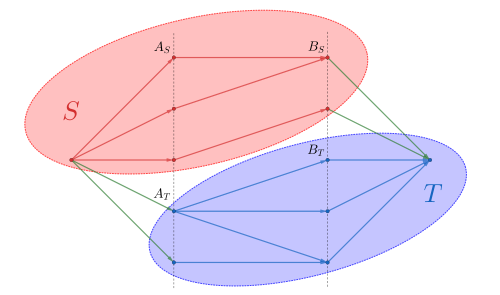
\includegraphics[width=0.6\textwidth]{imgs/mvc.png}
    \end{center}
\end{frame}
\subsection{ Matching Ponderado Bipartito Máximo }

\begin{frame}{Matching Máximo Bipartito Ponderado}
    Si al grafo bipartito $G$ le agregamos pesos en las aristas, podemos definir el peso de un matching como la suma de los pesos de las aristas utilizadas en él.

    Entonces, podemos buscar, entre los matchings de tamaño máximo, aquel que maximice o minimice el peso total.

    Esto puede alcanzarse de 2 formas:

    \begin{enumerate}
        \item Agregando el peso de las aristas a la red de flujo y utilizando Min Cost Max Flow en $O(|E|*|f|)$
        \item Algoritmo Hungaro: $O(|V|^3)$, con mejor constante que el algoritmo de flujo.
    \end{enumerate}
\end{frame}

\section{Partición de DAG en Caminos}
    \subsection{Partición en Cadenas}
    \begin{frame}{Partición de un DAG en caminos}
        
        \begin{definition}
           Sea un DAG $G = (V,E)$, podemos buscar una partición de sus nodos en caminos disjuntos. Es decir, buscar caminos $C_1, C-2, ..., C_k \in G$ tales que $V = \bigcup_{i=1}^k V(C_i)$ y $C_i \cap C_j = \emptyset$ para todo $i \neq j$.
        \end{definition}
        
        También podemos buscar una partición no necesariamente disjunta. Esta va a ser equivalente a una partición en caminos disjuntos de la clausura transitiva de $G$, y es así como la vamos a calcular.

        El problema consiste en buscar una partición en caminos de tamaño mínimo, es decir, con la mínima cantidad de caminos.
    \end{frame}

    \begin{frame}{Reducción a un problema de Matching Máximo}
        Sea un DAG $G = (V,E)$, para encontrar su mínima partición en caminos disjuntos, podemos reducirlo al problema de Matching Máximo Bipartito:
        \begin{enumerate}
            \item Defino un nuevo grafo bipartito $G' = (V', E')$
            \item Para cada nodo $v \in V$, agrego dos nodos $v_{in}, v_{out} \in V'$.
            \pause
            \item Para cada arista $(u,v) \in E$, agrego una arista $(u_{out}, v_{in}) \in E'$. 
            \pause
            \item Calculo el Matching Máximo Bipartito $M$ en $G'$.
            \item El tamaño de la mínima partición en caminos será $|V|-|M|$.
            \pause
            \item Las aristas que se usan en los caminos de la partición son las aristas del matching.
            \item Para saber donde empiezan los caminos, tomamos los $v$ tales que $v_{in}$ no está matcheado.
        \end{enumerate}    
    \end{frame}
\subsection{Teorema de Dilworth}
    \begin{frame}{Teorema de Dilworth}
        \begin{definition}{Anticadena}
            Sea un DAG $G = (V,E)$, una \textbf{anticadena} es $V' \subseteq V$ tal que no hay dos nodos $u,v \in V'$ tales que $u$ puede alcanzar a $v$ en $G$.
        \end{definition}
        
        \pause

        \begin{Theorem}[Dilworth]
            Sea un DAG $G = (V,E)$ y $C$ su mínima covertura en cáminos \textbf{no disjuntos}, el tamaño de la máxima anticadena $A$ es $|C|$.
        \end{Theorem}
        
    \end{frame}

    \begin{frame}{Teorema de Dilworth: Reconstrucción}
        Para reconstruir la máxima anticadena $A$ de un DAG $G = (V,E)$, podemos:
        \begin{enumerate}
            \item Construimos la clausura transitiva de $G$, $G' = (V,E')$.
            \pause
            \item Definimos el grafo bipartito $B = (V_B,E_B)$, donde $V_B = \{v_{in}, v_{out} : v \in V\}$ y $E_B = \{(u_{out}, v_{in}) : (u,v) \in E'\}$.
            \pause
            \item Calculamos un MVC $M$ de $B$.
            \pause
            \item Una máxima anticadena $A$ de $G$ es el conjunto de nodos $v \in V$ tales que $v_{in} \not \in M \wedge v_{out} \not \in M$
        \end{enumerate}
    \end{frame}

\section{Problemas de Maquinas y Tareas}

\subsection{Problema de Asignación}

\begin{frame}{Problema de Asignación}
    Sea un conjunto $T$ de tareas y un conjunto $M$ de máquinas necesarias para realizar la tarea:
    \pause
    \begin{itemize}
        \item Para comprar la máquina $m \in M$ necesitamos pagar un costo $c(m)$.
        \pause
        \item Para realizar la tarea $t \in T$ necesitamos un conjunto $M_t \subseteq M$ de máquinas.
        \pause
        \item Puedo utilizar una misma máquina para realizar cualquier cantidad de tareas, pero no puedo realizar una tarea si no tengo todas las máquinas necesarias.
        \pause 
        \item Si realizo la tarea $t$ obtengo un beneficio $b(t)$.
    \end{itemize}
    \pause 
    Quiero elegir un subconjunto de máquinas $M'$ a comprar y uno de tareas $T'$ a realizar, de tal forma que maximicemos el beneficio total neto.

    $$
    \max_{M' \subseteq M, T' \subseteq T, T'\text{ es posible dado }M'} \left( \sum_{t \in T'} b(t) - \sum_{m \in M'} c(m) \right)
    $$
\end{frame}

\begin{frame}{Reducción al problema de corte mínimo}
    Para resolver este problema, lo podemos reducir al problema de corte mínimo de la siguiente manera:
    \pause 
    \begin{enumerate}
        
        \item Asumo que ya me pagaron todos las tareas. Entonces, no realizar la tarea $t$ tiene un costo $b(t)$.
        
        \pause 

        \item Defino un grafo $G = (V,E)$
        \item Agrego un nodo fuente $S$ y un nodo sumidero $T$.
        \item Para cada máquina $m \in M$, agrego una arista $(S,m)$ con capacidad $c(m)$.
        \item Para cada tarea $t \in T$, agrego una arista $(t,T)$ con capacidad $b(t)$.

        \pause
        \item Para cada tarea $t \in T$ y cada máquina $m \in M_t$, agrego una arista $(m,t)$ con capacidad $\infty$.
        
        \pause
        \item Calculo el corte mínimo entre $S$ y $T$ en $G$.
        \item El máximo beneficio alcanzable es $\sum_{t \in T} b(t)$ menos el costo del corte mínimo. Esto representa la necesidad de la maquina $m$ para la tarea $t$.
        
        \pause
        \item Si la arista $(S,m)$ forma parte del corte, compro la máquina $m$.
        \item Si la arista $(t,T)$ forma parte del corte, entonces no realizo la tarea $t$.
    \end{enumerate}    
\end{frame}

\subsection{Generalización}

\begin{frame}{Generalización del problema de asignación}
    Sea $G = (V,E)$ un grafo dirigido y una función de valor $w:E \to \mathbb{Z}$, queremos elegir un subconjunto de nodos $V' \subseteq V$ tal que:
    \begin{enumerate}
        \item $\forall (u,v) \in E, v \in V' \implies u \in V'$.
        \item Maximiza $\sum_{v \in V'} w(v)$
    \end{enumerate}

    \pause
    Para resolver este problema construimos un grafo $G' = (V', E')$:
    \begin{enumerate}
        \item $V' = V \cup \{S, T\}$, donde $S$ es el nodo fuente y $T$ es el nodo sumidero.
        \pause
        \item Para cada nodo $v \in V$, si $w(v) < 0$, agrego una arista $(S,v)$ con capacidad $-w(v)$, y si $w(v) > 0$, agrego una arista $(v,T)$ con capacidad $w(v)$.
        \pause
        \item Para cada arista $(u,v) \in E$, agrego una arista $(u,v) \in E'$ con capacidad $\infty$.
        \pause
        \item Calculo el corte mínimo entre $S$ y $T$ en $G'$.
        \pause
        \item El conjunto de nodos $V'$ alcanzables desde $S$ en la red residual.
        \item El valor de $V'$ es la suma de los $w(v)$ positivos menos el corte minimo.
    \end{enumerate}

\end{frame}

\section{Trucos varios }

\begin{frame}{Capacidad en los nodos}
    Si necesitamos que los nodos $v \in V$ tengan una capacidad $c(v)$, podemos separar cada nodo $v$ en $v_{in}, v_{out}$ y :
    \begin{itemize}
        \item Reemplazar cada arista $(u,v) \in E$ por la arista $(u_{out}, v_{in})$ con capacidad $c(u,v)$.
        \item Agregar para cada nodo $v$ una arista $(v_{in}, v_{out})$ con capacidad $c(v)$. 
    \end{itemize}
\end{frame}
    
% \subsection{ Aristas con flujo mínimo }

\begin{frame}{Aristas con flujo mínimo}
    Sea $G = (V,E)$ un grafo dirigido con nodos sumidero $S$ y $T$, y funciones de flujo mínimo y máximo $c,d: E \to \mathbb{N}$.
    Queremos:
    \begin{enumerate}
        \item Decidir si es posible asignar un flujo $f: E \to \textbf{N}$ tal que $c(e) \leq f(e) \leq d(e) \forall e \in E$ y $\forall v \in V - \{S,T\}, \sum_{u: (u,v) \in E} f(u,v) = \sum_{w: (v,w) \in E} f(v,w)$.
        \item Si es posible, encontrar un flujo $f$ que cumpla lo anterior y maximice el valor $|f|$.
    \end{enumerate}
\end{frame}

\begin{frame}{Aristas con flujo mínimo - Solución}
    Para resolver este problema:
    \begin{enumerate}
        \item Construimos un grafo $G' = (V', E')$ donde $V' = V \cup \{S', T'\}$, nuevos nodos fuente y sumidero.
        \pause
        \item Para cada $(u,v) \in E$, agregamos a $E'$ una arista $(u,v)$ con capacidad $d(u,v) - c(u,v)$, arista $(S',v)$ y $(u,T)$, ambas con capacidad $c(u,v)$.
        \pause
        \item Agregamos aristas $(S',S)$ y $(T,T')$ con capacidad $\infty$.
        \item Calculamos el un flujo máximo $f'$ de $S'$ a $T'$. Si hay aristas salientes de $S'$ (excepto $(S',S)$) que no esten saturadas, el flujo no es satisfasible.
        \pause 
        \item Si el flujo es satisfasible, $f(u,v) = c(u,v) + f'(u,v)$ para cada $(u,v) \in E$.
        \item El flujo $f$ cumple las condiciones del problema y maximiza el valor $|f|$.
    \end{enumerate}
\end{frame}

\end{document}